% Compact PGFPlots panel for sampled surface7 BSC GEXIT derivative.
% Requires \usepackage{pgfplots} and \pgfplotsset{compat=1.18}.
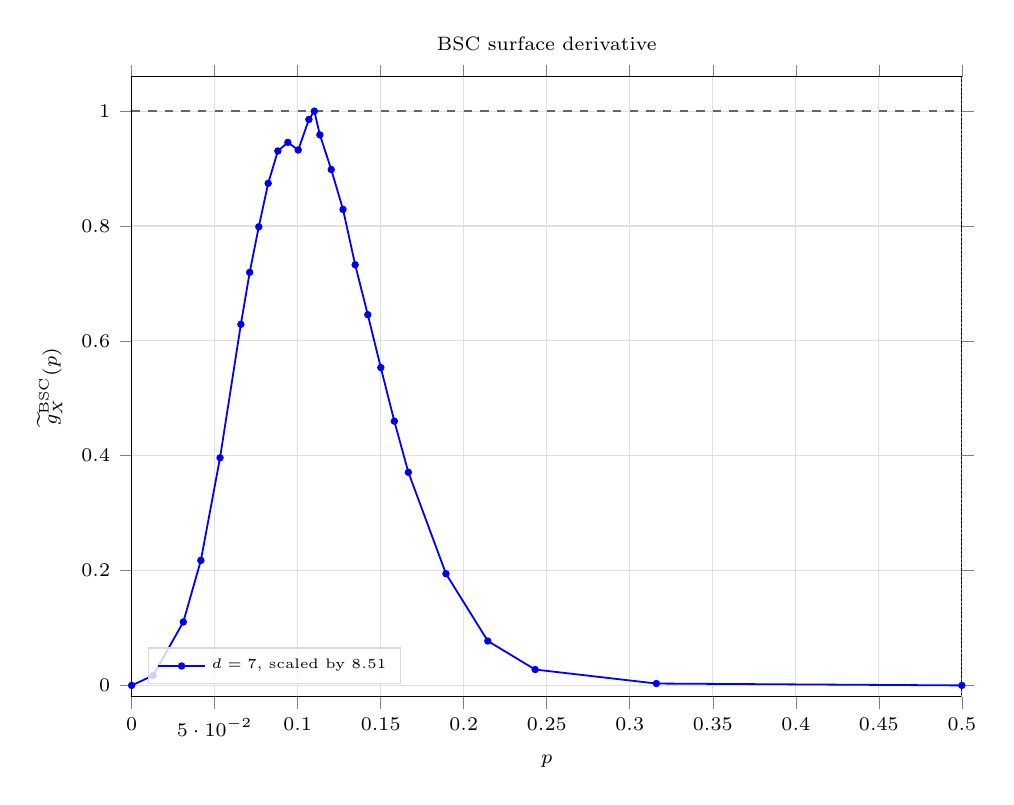
\begin{tikzpicture}
\begin{axis}[
  name=scaledBSCGEXITSurface7Axis,
  width=\linewidth,
  height=0.78\linewidth,
  title={BSC surface derivative},
  title style={font=\scriptsize},
  xlabel={$p$},
  ylabel={$\widetilde g_X^{\rm BSC}(p)$},
  xmin=0, xmax=0.5,
  ymin=-0.02, ymax=1.06,
  grid=both,
  major grid style={black!12},
  minor grid style={black!6},
  tick align=outside,
  tick label style={font=\scriptsize},
  label style={font=\scriptsize},
  legend cell align={left},
  legend style={draw=black!15, fill=white, fill opacity=0.82, text opacity=1, at={(0.02,0.02)}, anchor=south west, font=\tiny},
]
\addplot[black!60, densely dotted, line width=0.55pt, forget plot] coordinates {(0.5,-0.02) (0.5,1.06)};
\addplot[black!60, dashed, line width=0.55pt, forget plot] coordinates {(0,1) (0.5,1)};
\addplot+[color=blue, mark=*, mark size=1.0pt, line width=0.65pt]
coordinates {(0,0) (0.0129868620555,0.0173816081774) (0.0311244603048,0.110521856641) (0.0416926902737,0.21775458126) (0.0532390407768,0.396409798346) (0.0657867063546,0.628889065868) (0.0710958755299,0.719379415735) (0.0765765344037,0.798697965657) (0.0822333323659,0.874337861385) (0.0880715694979,0.930651872794) (0.0940972433461,0.945651041763) (0.100317108961,0.932360112032) (0.106738753821,0.985522590024) (0.110027864438,1) (0.113370689941,0.958702930052) (0.120222466333,0.898364879244) (0.127304805976,0.828907895046) (0.134629772869,0.732500289128) (0.142210976498,0.645616897255) (0.150063823499,0.553479923689) (0.158205829694,0.460122599201) (0.166657010397,0.371188406167) (0.189297705371,0.194516066418) (0.21450174486,0.077369516271) (0.243003853809,0.0276652066476) (0.316019346324,0.00327312562519) (0.5,0)};
\addlegendentry{$d=7$, scaled by $8.51$}
\end{axis}
\end{tikzpicture}
